\documentclass{ximera}

\title{Linear Algebra}

\begin{document}
\begin{abstract}
The linear algebra portion of the self-evaluation test for the
University of Leuven's Masters of Artificial Intelligence program.
\end{abstract}
\maketitle

% Question 33
\begin{question}
True or false?  When the dot product of two vectors is negative, the angle between them is between 90 and 270 degrees.
\begin{solution}
\begin{multiple-choice}
\choice[correct]{true}
\choice{false}
\end{multiple-choice}
\end{solution}
Since the lengths of two vectors are always non-negative, a negative dot product indicates an angle with negative cosine. The range of angles with a negative cosine are those between 90 and 270 degrees.
\end{question}

% Question 34
\begin{question}
Given the vectors $u$ and $v$, give a matrix $M$ that transforms them
into $u'$ and $v'$; that is, find $M$ such that $M u=u'$ and $M v=v'$.
% TODO (Behrouz) the vectors in this image should be transposed
% TODO (Behrouz) use pgfplots instead of including an image
\begin{image}
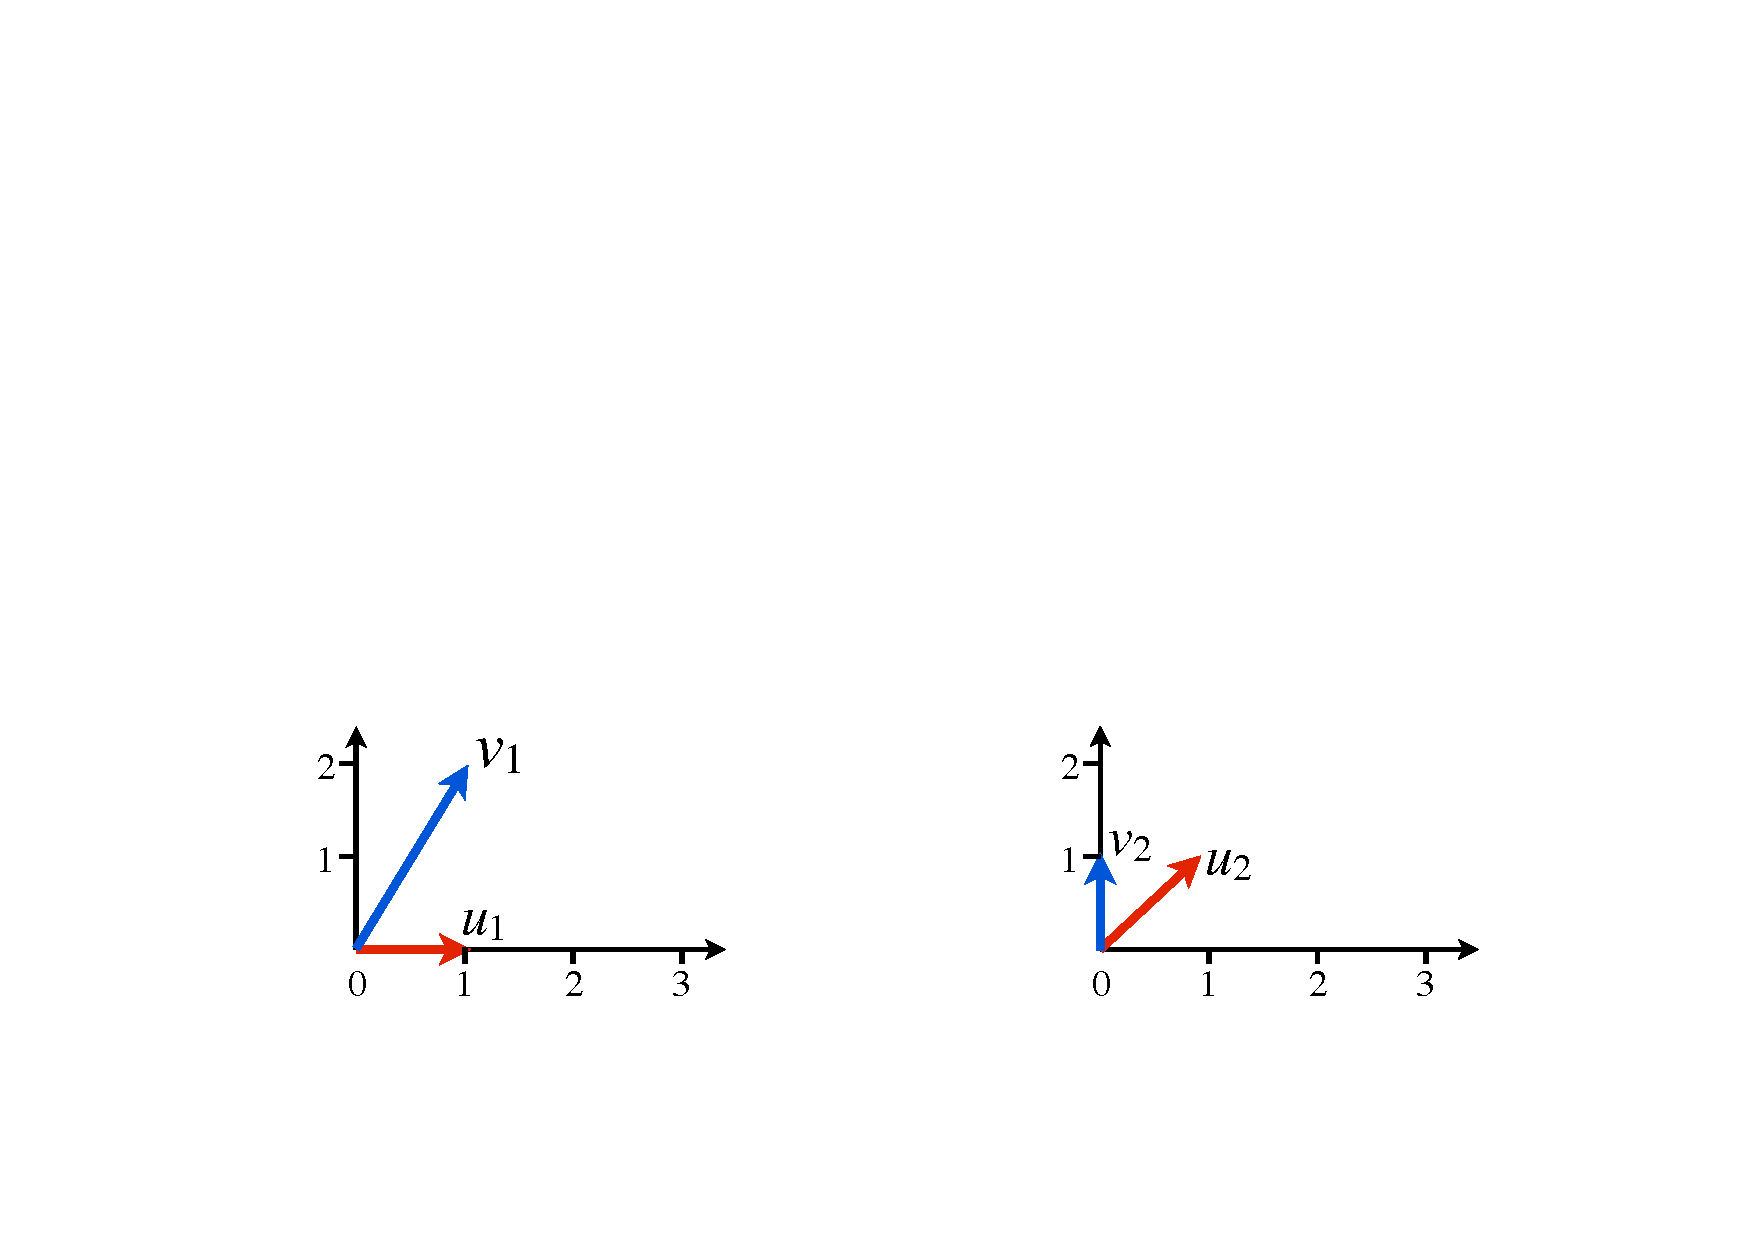
\includegraphics[width=0.6\textwidth]{fig.pdf}
\end{image}
\end{question}

\end{document}
